% !TeX spellcheck = en_US
% !TeX root = ../Tom_Sandmann-master_thesis
\chapter{SAKURA-G} \label{chp: SAKURA-G}
\lettrine[lhang = 0.4, findent=-30pt, lines=4]{\textbf{
		\initfamily \fontsize{20mm}{20mm} \selectfont T
		\normalfont}}{he}
SAKURA-G board consists of two integrated Spartan-6 FPGAs.
One of these Spartan FPGAs serves as the main security circuit (XC6SLX75-2CSG484C), while the other one serves as the controller (XC6SLX9-2CSG225C). 
The main Spartan contains the actual cryptographic hardware design.
The control Spartan is used to control the main board by changing specific signals received by the main board (e.g. signals indicating whether encryption/decryption has to be performed, or whether the internal state has to be reset). 
To deploy a hardware design on our FPGA, we need to somehow transfer this design to the board.
This requires the hardware design to be processed in a specific way:
% https://www.xilinx.com/itp/xilinx10/isehelp/ise_c_implement_fpga_design.htm
\begin{enumerate}
	\item \textbf{Synthesis}: the abstract description of our hardware design (written in for example VHDL or Verilog) is turned into a design implementation of logic gates and lookup tables (LUTs), digital signal processors (DSPs), BRAMs and other elements.
	
	\item \textbf{Mapping, Place and Route}: the structures identified in the previous step are mapped to FPGA elements.
	These components are then routed and the appropriate signals are connected.
	
	\item \textbf{Program file}: a file is generated that can be transferred to the FPGA. Depending on the file format, this file either gets flashed to the flash memory on the SAKURA-G board, or is stored in the FPGA non-persistent memory.
\end{enumerate}
%

\section{Constraints}
Constraints are used to guide the design tool on how specific parts of the design should be treated. There are two types of constraints:
%
\begin{itemize}
	\item \textbf{Synthesis constraints} are used by the synthesis tool to optimize specific parts of the hardware description language (HDL) code. 
	They can be either embedded directly within the VHDL/Verilog code or specified in an external synthesis constraint file.
	
	\item \textbf{Implementation constraints} are instructions passed to FPGA implementation tools that specify mapping, placement, timing and other guidelines followed by the implementation tool while processing a FPGA design. These constraints are generally placed in a User Constraint File (\texttt{UCF}). Examples of these constraints are \texttt{LOC} (placement) and \texttt{PERIOD} (timing) constraints. In the hardware design we consider, the majority of the constraints (if not all) are \texttt{LOC} constraints. \texttt{LOC} constraints define where a design element can be placed within a FPGA. 
\end{itemize}
%

\section{JTAG}
JTAG was a standard initially developed by IEEE to solve issues with electronically manufactured boards. 
It is a standard used to verify designs and circuit board after they have been manufactured.
In our case, it is used as a programming, debug and probing port. 
The JTAG programmer/debugger is attached to both the JTAG port and the micro-USB port, which makes it ready to use. 
We use the JTAG programmer to load hardware designs of the control and main FPGAs to the Spartan FPGAs.
In general, there are two file formats that can be loaded to a FPGA:
%
\begin{itemize}
	\item \texttt{BIT} file: A \texttt{.BIT} file is a raw storage of the programming bits for the FPGA.
	It can be loaded to the FPGA via JTAG using for example \texttt{iMPACT} (a Xilinx specific utility).
	This file format is primarily used for testing a hardware design. The reason for this is, when the board loses its power, the design is ``lost''.
	
	\item \texttt{MCS} file: A \texttt{.MSC} file is flashed to flash memory, which means that the contents are not lost when power is lost. The \texttt{.MSC} file can be flashed to flash-memory via JTAG using \texttt{iMPACT}. On power-up, specific configuration signals are used to load the program to the board.
\end{itemize}
%

% !TeX spellcheck = en_US
% !TeX root = ../Tom_Sandmann-master_thesis
\section{Interface with the board} \label{sec: Interface with the board}
To interface with the Spartan FPGAs that are present on the SAKURA-G, we make use of Python code from the ChipWhisperer project%
\footnote{\url{https://newae.com/tools/chipwhisperer/}}.
In addition, we make use of the source files for both the main and control FPGAs available on the SAKURA-G website%
\footnote{\url{http://satoh.cs.uec.ac.jp/SAKURA/hardware/SAKURA-G.html}}.
The software needed to develop and deploy hardware designs to our board is as follows:
%
\begin{itemize}
	\item Xilinx ISE 14.7 (licensed);
	\item FTDI drivers D2XX%
	\footnote{\url{http://www.ftdichip.com/Drivers/D2XX.htm}};
	\item FT PROG%
	\footnote{\url{http://www.ftdichip.com/Support/Utilities.htm\#FT_PROG}}.
\end{itemize}
%
The FTDI drivers are required by the \texttt{ftd2xx} Python package to send and receive data to and from one of the FPGAs (i.e. either the control or the main FPGA).
\mintinline{text}{FT_PROG} can be used to view connected FPGAs (if any).
Finally, Xilinx ISE is used to generate the corresponding program files for our design and send them to the board. 

We now describe the structure of the interfaces used in the designs of the control and main FPGAs.
The two FPGAs on the SAKURA-G board are interconnected through a local bus.
The SAKURA-G makes use of an USB FTDI interface that allows an external PC to communicate with the one of the FPGAs.
Channel A of the the USB interface (FT2232H) is connected to the controller FPGA and channel B is connected to the main FPGA.
Depending on the DIP switch (and another control flag), we are connected to either the main FPGA or to the control FPGA.
As we do not need to directly interface with the main FPGA, we assume to be always connected to the USB interface of the control FPGA.

The control FPGA can send and receive data to the main FPGA by making use of the local bus.
The control FPGA also receives external inputs such as a 48MHz clock and a reset signal.
In addition, it can also control the LEDs that are located next to the FPGA on the board.
The 48MHz clock that is received as input by the control FPGA is used to generate two clocks:
one that is used as the system clock (\texttt{clk}), and another one (\mintinline{text}{usb_clk}) to clock the USB connection (which by default is clocked at 24MHz).
The system clock is used in both the local bus (connecting the two FPGAs) and in the main FPGA.
The frequency at which the system clock operates is controlled by the (4-bit wide) User DIP switch (where the default operation frequency is 1.5MHz).
To make use of a different operation frequency, we set the first bit of the DIP switch to high.
The remaining bits of this switch control the new frequency (3, 6, 12 or 24MHz).
A schematic overview of the connection between the two boards can be seen in \Cref{fig: sakura_g-signal-overview}.
%
\begin{figure}
	\centering
	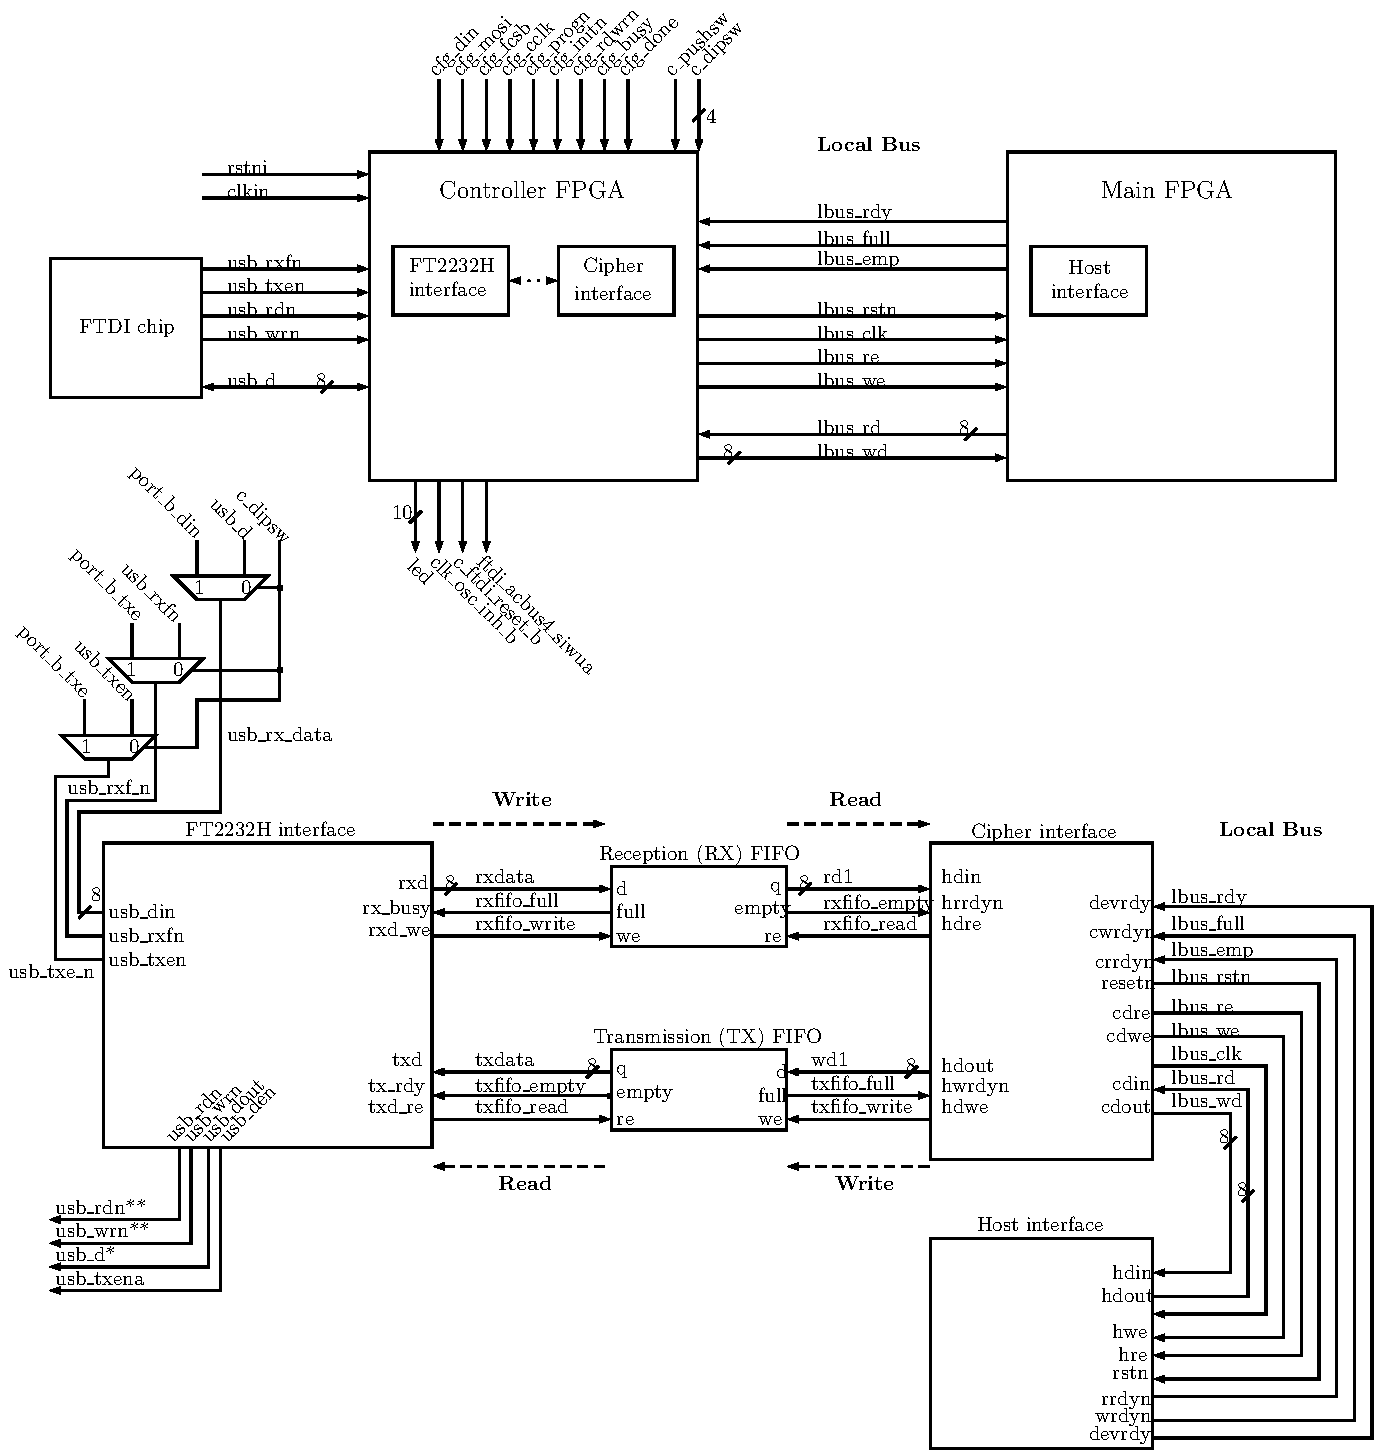
\includegraphics[scale=0.65]{sakura_g-signal-overview}
	\captionof{figure}{Overview of the interfaces used by both the main and control FPGAs. The control FPGA only moves data between the USB port and the control FPGA (via the FT2232H interface) and between the main FPGA and the control FPGA (via the Cipher interface).
	Data transmission between the Cipher interface and the FT2232H interface is done by making use of two FIFOs: a transmission (TX) and a reception (RX) FIFO. 
	The TX FIFO is used to transport data (written by the) Cipher interface to the FT2232H interface,
	while the RX FIFO is used to transport data from the FT2232H interface to the Cipher interface.
	Note that not all input signals are shown (e.g. the clock and reset signals for both FIFOs are omitted).
	The meaning of the single and double stars in some of the output signals from the FT2232H interface are as follows:\\
	%
	\textbf{*}: The value of \mintinline{text}{usb_d} contains the value that is read from the TX FIFO if the first bit of the DIP switch is low (i.e. \mintinline{text}{c_dipsw(0) = '0'})  (and when \mintinline{text}{usb_txena = '1'}). \\
	\textbf{**}: The value of \mintinline{text}{usb_rdn (usb_wrn)} equals the internal \mintinline{text}{usb_rdn (usb_wrn)} signal when the first bit of the DIP switch is low (i.e. \mintinline{text}{c_dipsw(0) = '0'}), otherwise it is a constant value of 1.
	}
	\label{fig: sakura_g-signal-overview}
\end{figure}
%
\begin{figure}
	\centering
	% !TeX spellcheck = en_US

\begin{tikzpicture}[->, >=stealth',shorten >=1pt,auto,node distance=2cm]
\node[state, initial] (idle) {$i$};

\node[state, above right of = idle] (read1) {$r_1$};
\node[state, right of = read1] (read2) {$r_2$};
\node[state, right of = read2] (read3) {$r_3$};

\node[state, below right of = read3] (back off) {$b$};

\node[state, below right of = idle] (write1) {$w_1$};
\node[state, right of = write1] (write2) {$w_2$};
\node[state, right of = write2] (write3) {$w_3$};

\draw (idle) edge[bend left, above] node[align=left, xshift=-40pt]{\mintinline{text}{usb_rxf_reg = '1'} \\ \mintinline{text}{rx_busy = '0'}} (read1);

\draw (idle) edge[bend right, below] node[align=left, xshift=-40pt, yshift=-10]{\mintinline{text}{usb_txe_reg = '1'} \\ \mintinline{text}{tx_rdy = '0'}} (write1);

\draw (read1) edge node{} (read2);
\draw (read2) edge node{} (read3);
\draw (read3) edge[bend left, below] node{} (back off);

\draw (back off) edge node{} (idle);

\draw (write1) edge node{} (write2);
\draw (write2) edge node{} (write3);
\draw (write3) edge[bend right, below] node{} (back off);

\draw (idle) edge [loop above, left, in=-30, out=30, looseness=5] (idle);
\end{tikzpicture}

	\captionof{figure}{Finite state machine used by the FT2232H interface to control the reading and writing from the FTDI USB chip. In the read states ($r_1, r_2, r_3$), a single byte is received from the USB channel in order to be sent to the main FPGA. In the write states ($w_1, w_2, w_3$), a single byte is transmitted over the USB channel.}
	\label{fig: usb_fsm}
\end{figure}
%
We give a short description for each of the interfaces:
%
\begin{itemize}
	\item \textbf{FT2232H interface}: this component reads data from the USB port (FTDI based) and writes in the internal reception FIFO (RX). 
	In addition, it also reads the transmission FIFO (TX) and sends it to the USB port (\Cref{fig: sakura_g-signal-overview}).
	Reading and writing from the FTDI chip is controlled by a finite state machine (FSM) (\Cref{fig: usb_fsm}).  
	This FSM starts in the idle state $(i)$, in which it is determined whether it can start to read data from the USB channel ($r_1$), write data to the USB channel ($w_1$) or remain in the idle state $(i)$. 
	We describe the read and write states in more detail:
	%
	\begin{itemize}
		\item \textbf{Read}. 
		If the RX FIFO is ready and not busy (\mintinline{text}{usb_rxf_reg = '1'} and \mintinline{text}{rx_busy = '0'} respectively), we proceed to the first read state ($r_1$). 
		Once we are in the second read state $(r_2)$, we read the actual byte from the USB channel, and set the write enable of the RX FIFO and indicate that this register is read ready. 
		Finally we proceed to the final read state $(r_3)$, in which the data read from the USB channel is actually written into the RX FIFO. 
		After resetting the write enable of the RX FIFO, we proceed to the back-off state $(b)$.
		
		\item \textbf{Write}.
		If the TX FIFO is ready (\mintinline{text}{usb_txe_reg = '1'} and \mintinline{text}{tx_rdy = '1'}), we proceed to the first write state $(w_1)$.
		In the first write state $(w_1)$, we reset the read enable of the TX FIFO and enable the output of the USB data bus. 
		In the second write state $(w_2)$, we indicate that the value from the TX FIFO is ready to be written to the USB port. 
		
		\item \textbf{Back off}.
		In the back off state $(b)$, we reset the USB write enable (which is low active).
		This signal is passed to the FTDI chip, which then knows that it can set the corresponding signals to send another byte.
		In addition, we also reset the output-enable signal (which indicates whether the output data is valid or not).
		
	\end{itemize}
	%
	\item \textbf{Cipher interface}: This is the interface with the main FPGA. This component controls the local bus between the control and the main FPGA.
	It reads the reception FIFO (RX) that the FT2232H interface writes, and writes content received from the local bus (i.e. written by the host interface) into the transmission (TX) FIFO (see \Cref{fig: sakura_g-signal-overview}).
	Reading and writing from the main FPGA (i.e. the host interface) is controlled by two state machines: 
	%
	\begin{figure}
		\centering
		\subfloat[Finite state machine used by the cipher interface to control the reading from the data written on the local bus by the host interface (i.e. main FPGA).]{
			% !TeX spellcheck = en_US

\begin{tikzpicture}[->, >=stealth',shorten >=1pt,auto,node distance=3cm]
\node[state, initial] (idle) {$i$};

\node[state, right of = idle] (read) {$r$};

\draw (idle) edge[bend left, above] node[align=left]{\mintinline{text}{devrdy = '1'} \\ \mintinline{text}{hwrrdyn = '0'} \\ \mintinline{text}{crrdyn = '0'}} (read);

\draw (idle) edge [loop above, left, out=-60, in=-120, looseness=5] (idle);

\draw (read) edge [bend left, below] (idle);

\end{tikzpicture}

			\label{subfig: cipher read fsm}
		}
		\hspace{0.5cm}
		\subfloat[Finite state machine used by the cipher interface to control the writing to the local bus connected to the main FPGA.]{
			% !TeX spellcheck = en_US

\begin{tikzpicture}[->, >=stealth',shorten >=1pt,auto,node distance=3cm]
\node[state, initial] (idle) {$i$};

\node[state, right of = idle] (fifo read) {$r$};

\node[state, right of = fifo read] (lbus write) {$w$};

%\draw (idle) edge[bend left, above] node[align=left]{\mintinline{text}{hwrdyn = '0'} \\ \mintinline{text}{crrdyn = '0'}} (read);

\draw (idle) edge [loop above, left, out=-60, in=-120, looseness=5] (idle);
\draw (idle) edge node[align=left, yshift = 15] {\mintinline{text}{hwrdyn = '0'} \\ \mintinline{text}{crrdyn = '0'}} (fifo read);
\draw (fifo read) edge (lbus write);
\draw (lbus write) edge[loop above, left, out=120, in=60, looseness=5] node[xshift=30, yshift=10] {\mintinline{text}{cwrdyn = '1'}} (lbus write);
\draw (lbus write) edge [bend left, below] node[align=left]{\mintinline{text}{cwrdyn = '0'}} (idle);

\end{tikzpicture}

			\label{subfig: cipher write fsm}
		}			
		\captionof{figure}{State machines used by the cipher interface to control the reading from and writing to the host Interface.}
		\label{fig: cipher_rw_fsm}
	\end{figure}
	%
	\begin{itemize}
		\item \textbf{Cipher Read} (\Cref{subfig: cipher read fsm}): This state machine controls the reading from data that is written on the local bus by the host interface. The FSM starts in the idle state ($i$), in which it waits until the main FPGA is ready, the host interface is write ready and the cipher interface is read ready (see \Cref{subfig: cipher read fsm}). If this is the case, the FSM moves to the read state $(r)$. In addition, it sets the read enable and clears the write enable of the host. In the read state, the input received over the local bus (\mintinline{text}{lbus_rd}) is written to the TX FIFO. The values of the cipher read and host write enable are restored to their original values.		
			
		\item \textbf{Cipher Write} (\Cref{subfig: cipher write fsm}): This state machine controls the writing on the local bus, which is read by the host interface. The FSM starts in the idle state $(i)$, in which it waits until the host interface is write ready, and the cipher interface is read ready. If this is the case, the FSM moves to a read state in which it reads data from the Reception (RX) FIFO. In the write state, this data is then transmitted over the local bus such that it can be read by the host interface.
	\end{itemize}
	%
	\item \textbf{Host interface}: This component reads and writes the local bus between the control and the main FPGA. It is mainly a state machine. It controls the implementation through the values that are written in the bus. 
	Received values are stored in registers.
	Depending on the received value and the appropriated control signals (e.g. write enable (WE)), parts of the register are assigned specific values.
	This component consists of two registers: \mintinline{shell}{addr_reg} and \mintinline{shell}{data_reg}. 
\end{itemize}
%
% !TeX spellcheck = en_US
% !TeX root = ../Tom_Sandmann-master_thesis

\section{IP blocks} \label{sec: IP Blocks}
The hardware design of {\fourq} \cite{jarvinen2016four} (\Cref{chp: FourQ On Hardware}) makes use of a couple of Intellectual Property (IP) blocks provided by Xillinx.
An IP block is a reusable unit of logic, which is the intellectual property of one party.
The IP blocks, and their corresponding configurations, used within the {\fourq} hardware design are as follows:
%
\begin{itemize}
	\item \textbf{\mintinline{text}{blk_mem_gen_0}}: \\ Memories \& Storage Elements $\to$ RAMs \& ROMs \& BRAMs $\to$ Block Memory Generator
	\begin{table}[H]
		\centering
		\begin{tabular}{cc}
			\toprule
			\textbf{Setting} & \textbf{Value} \\
			\midrule
			Memory type & True Dual-Port RAM \\
			Clocking Options & Common Clock \\
			Port A/B Write Width & 128 \\
			Port A/B Write Depth & 256 \\
			Port A/B Enable & Use ENA/ENB Pin \\
			Port A/B & Register Port A/B output of Memory Primitives \\
			All other options & Keep defaults \\
			\bottomrule
		\end{tabular}
	\end{table}
	%
	\item \textbf{\mintinline{text}{blk_mem_gen_1}}: \\ Memories \& Storage Elements $\to$ RAMs \& ROMs \& BRAMs $\to$ Block Memory Generator
	\begin{table}[H]
		\centering
		\begin{tabular}{cc}
			\toprule
			\textbf{Setting} & \textbf{Value} \\
			\midrule
			Memory type &  Single Port ROM\\
			Algorithm & Fixed Primitives $\to$ Primitive (Write Port A): 1kx18 \\
			Port A Write Width & 25 \\
			Port A Write Depth & 8192 \\
			Port A Enable & Use ENA Pin\\
			Port A & Register Port A output of Memory Primitives \\
			Load Init file & \mintinline{text}{prog_code.coe} \\
			All other options & Keep defaults \\
			\bottomrule
		\end{tabular}
	\end{table}
	%
	\item \textbf{\mintinline{text}{mult_gen_0}}: \\ Math Functions $\to$ Multipliers $\to$ Multiplier
	\begin{table}[H]
		\centering
		\begin{tabular}{cc}
			\toprule
			\textbf{Setting} & \textbf{Value} \\
			\midrule
			Port A/B data type & Unsigned \\
			Port A/B width & 64 \\
			Multiplier Construction & Use Mults \\
			Pipeline stages & 7 \\
			All other options & Keep defaults \\
			\bottomrule
		\end{tabular}
	\end{table}
	%
\end{itemize}
%

% !TeX spellcheck = en_US
% !TeX root = ../Tom_Sandmann-master_thesis
\section{Reading and writing of internal registers}
The hardware design of {\fourq} requires us to first load specific constants into the RAM.
These constants are used during the scalar multiplication, and reduce the number of computations necessary.
In \Cref{chp: FourQ}, we describe these constants in more detail.
After the constants are loaded into RAM, the design can be controlled by specific operations.
These operations are described in \Cref{subsec: Control Logic}.
To control data assignment to the RAM, we make use of a FSM at the main FPGA.
This FSM can be seen in \Cref{fig: host fsm}.
%
\begin{figure}
	\centering
	% !TeX spellcheck = en_US

\begin{tikzpicture}[->, >=stealth',shorten >=1pt,auto,node distance=2cm]
\node[state, initial] (cmd) {$i$};
\draw (cmd) edge [loop above, left, in=60, out=120, looseness=5] (cmd);

\node[state, right of = cmd] (write addr msb) {$w_1$};
\node[state, right of = write addr msb] (write addr lsb) {$w_2$};
\node[state, right of = write addr lsb ] (write data msb) {$w_3$};
\node[state, right of = write data msb ] (write data lsb) {$w_4$};

\node[state, below of = write addr lsb] (wait read effective) {$r_{wait}$};
\node[state, right of = wait read effective] (read data msb) {$r_3$};
\node[state, right of = read data msb ] (read data lsb) {$r_4$};


\draw (cmd) edge node{} (write addr msb);
\draw (write addr msb) edge node{} (write addr lsb);
\draw (write addr lsb) edge node{} (wait read effective);
\draw (wait read effective) edge [loop above, left, in=150, out=210, looseness=5] (wait read effective);
\draw (wait read effective) edge node{} (read data msb);
\draw (read data msb) edge node{} (read data lsb);

\draw (write addr lsb) edge node{} (write data msb);
\draw (write data msb) edge node{} (write data lsb);

\draw (write data lsb) edge [bend right, above] node{} (cmd);

\draw (read data lsb) edge [bend left=50] node{} (cmd);

\end{tikzpicture}

	\captionof{figure}{Finite state machine used by the host interface to control the reading from and writing to the internal registers and control signals of the {\fourq} component.}
	\label{fig: host fsm}
\end{figure}
%
The FMS writes the \mintinline{text}{data_reg} and \mintinline{text}{addr_reg} values. 
Based on the values in these registers, the {\fourq} input signals are controlled.
We describe the FSM of \Cref{fig: host fsm} in more detail.
In both the reading and writing states, first the value of the address is transmitted  $(w_1, w_2)$ followed by a data read/write ($(r_3, r_4)$ or $(w_3, w_4)$ respectively).
Because values of both the address and data are 2 bytes, and we can only transmit one byte at a time, this transmission is done in two steps: the most significant byte (MSB) is sent first, followed by the least significant byte (LSB).
If the FSM is in the reading state and the address value has been transmitted, the address value is used to determine the output of the host interface.
This is realized by a multiplexer, where the value of the address determines which output signals are retrieved.
In the final design, reading from the main FPGA is primary used to retrieve the \texttt{busy} control signal, or (parts of) the result point of the scalar multiplication. 
The multiplexer can also be used to verify whether data assignments are done correctly within the interface itself.

The reason for the address to be 2 bytes is due to the size of the addresses within {\fourq} to load the RAM constants.
These addresses are 9 bits, where the first bit indicates whether we write the lower or upper half of the 128-bits value.
The remaining 8 bits specify the value of the address.
Fortunately, these data and address sizes are also used in the example main FPGA design that comes with the SAKURA-G, and required (almost) no change.

If we want to write data values to the main FPGA, the address is used by the hardware design to control the assignment of data (which are transmitted after the address) to the correct range of a signal.
Once the address is transferred, 2 bytes of data are transmitted.
After this is done, a control signal indicates that the assignment of data to the address can be made. 
If the address is not known internally, all values keep their previous value.
In the case of reading, there is an additional state in the FSM which waits for the value-to-read to become available.
The reason for this is due to a read latency of five periods.
The first three periods in this latency are because of how the interface of the memory is done in the {\fourq} design.
The remaining two periods are due to the two pipeline stages when reading from the True Dual-Port RAM (TDPR).
In general, the latency for either of the ports of the TDPR can be seen in the corresponding Block Memory Generator (BMG) configuration (see \Cref{sec: Interface with the board}).

% !TeX spellcheck = en_US
% !TeX root = ../Tom_Sandmann-master_thesis
\section{Capturing power traces}
To perform side channel analysis of the {\fourq} hardware design on the FPGA, we need to obtain power traces as {\fourq} is calculating the scalar multiplication.
A power trace is a collection of samples.
Each sample is a tuple of voltage and time values.
Time values are represented in seconds (s), while the amplitude values are represented in volts (v).
To obtain power traces, the FPGA is connected to the oscilloscope.
The SAKURA-G is designed with ultra-low noise in mind.
The board provides a couple of SMA connectors that can be used to monitor the power waveforms. 
The board also comes with an on-board amplifier, which can used to monitor the amplified waveform (for both the control and main FPGAs).
To control the acquisition of a power trace, we make use of a trigger.
The trigger tells the oscilloscope when it should start the acquisition of a waveform (i.e. when the value of the trigger is high) and when this acquisition should stop (i.e. when the oscilloscope's memory is full). 
The oscilloscope used to display and retrieve the captured power traces is the Teledyne LeCroy - WaveRunner 610Zi.
To connect with the oscilloscope and retrieve the acquired waveforms, an Ethernet cable (ENET) was employed.
Teledyne LeCroy oscilloscopes employ a standard Ethernet interface for utilizing the TCP/IP transport layer \cite{automation2017manual}.
Other methods for making the remote connection exist as well (such as USBTMC, GPIB and LSIB).
To interface with the oscilloscope, we make use of ActiveDSO, which is an ActiveX control.
ActiveDSO provides interface drivers and a client library to make the remote connection over ENET, GPIB or USBTMC interfaces.
It also supports many automation features besides remote control. One can read more about how Teledyne LeCroy oscilloscopes can be controlled by a variety of Windows applications and programming languages in the ActiveDSO's developer guide \cite{activedso2015guide}.
As the interface with the SAKURA-G board is written in Python, this is also the language of choice for communicating with the oscilloscope.
In Python, the control object used to communicate with the oscilloscope is instantiated as follows:
%
\begin{minted}[xleftmargin=\parindent, tabsize=4, obeytabs, breaklines, fontsize=\footnotesize]{python3}
command = "LeCroy.ActiveDSOCtrl.1"
_scope = win32com.client.Dispatch(command)
\end{minted}
%
Using the control object, we can write commands to the oscilloscope and read back the response. To make this possible, we connect to the oscilloscope:
%
\begin{minted}[xleftmargin=\parindent, tabsize=4, obeytabs, breaklines, fontsize=\footnotesize]{python3}
ip_address="192.168.0.1"
command = "IP:" + ip_address
_scope.MakeConnection(command)
\end{minted}
%
The IP address should match the IP address set in the settings of the oscilloscope.
After establishing a connection with the oscilloscope, we can use the control object to send commands to the device.
ActiveDSO supports two types of commands that can be sent to the oscilloscope using the instantiated control.
Both traditional IEEE 488.2 (GPIB) commands and the Windows\textsuperscript{\textregistered} Component Object Model (COM) commands can be used.
Examples of these commands are as follows:
%
\begin{minted}[xleftmargin=\parindent, tabsize=4, obeytabs, breaklines, fontsize=\footnotesize]{python3}
# 488.2 format
scope.WriteString("<command string>", <Boolean EOI>)
# Automation Control within the VBS command
scope.WriteString("app.Shutdown", True)
\end{minted}
%
If End of Identify (EOI) is set to 1 (\mintinline{text}{True}), the command terminates with EOI, and the device interprets the command right away. This is normally the desired behavior.
If EOI is set to 0 (\mintinline{text}{False}), a command may be sent in several parts with the device starting to interpret the command only when it receives the final part.
This final command should have set its EOI value set to (\mintinline{text}{True}).
If a command string contains characters like double quotes ("), the command string should be surrounded with triple quotes.
Otherwise, Python would interpret the first double quote as the end of the command string, which is unintended.

The oscilloscope offers a variety of interfaces for using devices to input analog or digital signals. 
A series of connectors arranged on the front of the instrument are used to input analog signals on channels 1-4. 
We use these analog inputs to connect our FPGA to the oscilloscope. 
Each of these channels interfaces power probes and completely integrates the probe with the channel. 
When connected, the probe type is recognized and some setup information, such as input coupling and attenuation, is performed automatically.
Besides these analog inputs, one can also make use of probes and the LBUS interface.
In our setup, we only use the analog inputs to capture the power traces of our FPGA.
To get the waveform from a corresponding channel, we have to call the appropriate ActiveDSO method.
The available methods for acquiring a waveform can be seen in \cite{activedso2015guide}.
%
%\begin{itemize}
%	\item \texttt{GetByteWaveform}. This method reads raw 8-bit waveform data from the instrument into a byte array. Visual Basic's (unsigned) byte type (values between 0 and 255) is used to store the signed data bytes (values between -128 and 127) that the scope emits. 
%	To make this work, the signed data is `shifted' by 128, such that it can fit in the unsigned data type. 
%	This should be remembered when the data is scaled.
%	The \texttt{GetByteWaveform} method should be used when unscaled 8-bit waveform data is required. 
%	Processed waveforms are usually 16-bit waveforms. 
%	To avoid losing precision, they should be transmitted in 16 bit form. 
%	This can be done by making use of the \texttt{GetIntegerWaveform} method.
%	
%	\item \texttt{GetIntegerWaveform}. This method reads raw 16-bit waveform data from the instrument into an integer array. 
%	This method should be used when unscaled 16-bit waveform data is required. 	
%	Processed waveforms are usually 16-bit waveforms. 
%	To avoid losing precision, they should be transmitted in 16-bit format.
%	Channel waveforms are usually 8-bit waveforms. 
%	They may be transferred using the \texttt{GetByteWaveform} method. 
%	This reduces the time and storage requirements.
%	
%	\item \texttt{GetNativeWaveform}. This methods reads a waveform from the instrument in its native binary form. 
%	You can specify whether the data should be transmitted as 16-bit words or as regular 8-bit bytes.
%	A parameter for this method is also used to specify which entity of the waveform should be transmitted.
%	Possible values fort his parameter are the descriptor (DESC), the user text (TEXT), the time descriptor (TIME), the data block (DAT1), a second block of data (DAT2) or all entities (ALL).
%	As mentioned in the previous described methods, processed waveforms are usually 16-bit waveforms and should be captured by setting the word data argument to \mintinline{text}{True}.
%	Channel waveforms ($C_1, \ldots, C_4$) should be transmitted by setting the word data argument to \mintinline{text}{False}.
%	It is also possible to restore a waveform captured using the \texttt{GetNativeWaveform}.
%	This is only possible if the waveform was captured using the (ALL) parameter.
%	If this is the case, the \texttt{SetNativeWaveformSetNativeWaveform} can be used to restore the waveform.
%	
%	\item \texttt{GetScaledWaveform}. This method reads a scaled waveform from the instrument. 
%	The result is a scaled waveform stored as an array of single-precision floating point values.
%	If the time value corresponding to each sample amplitude is required, the \texttt{GetScaledWaveformWithTimes} method should be used.
%	
%	\item \texttt{GetScaledWaveformWithTimes}. This method reads a scaled waveform from the instrument and stores the time and amplitude at each sample point.
%	The result is a scaled waveform stored as a two-dimensional array of single-precision floating point values. In the first column, the time values are stored. In the second column, the amplitude values are stored.
%	If the time value corresponding to each sample amplitude is not required, one can use the \texttt{GetScaledWaveform} method.
%	
%\end{itemize}
%%

%If 16-bit words are send from the oscilloscope, we have to take the order in which the bytes for a single word are stored into account.
%To determine which byte order the oscilloscope is currently using waveform data transmission, we can make use of the \mintinline{text}{COMM_ORDER} command. 
%This command can be used to either ask for the current communication order or to set the communication order.
%When setting the communication order using the \mintinline{text}{COMM_ORDER} command, we use the following command syntax: \mintinline{text}{COMM_ORDER <mode>}, with \mintinline{text}{<mode> := {HI, LO}}.
%If \mintinline{text}{HI} is used, waveform data is sent with the most significant byte (MSB) first (i.e. big endian). 
%If \mintinline{text}{LO} is used, waveform data is sent with the least significant byte (LSB) (i.e. little endian).
%As we can read in the Remote Control Manual, data should be sent with the LSB first for Intel-based computers.
%For Motorola-based computers, data should be sent with the MSB first, the default at power-up. Data written to the instrument's hard disk, USB, or floppy always remains in LSB first format (the default DOS format). You cannot use the \mintinline{shell}{COMM_ORDER} command in these cases, since it is only meant for data sent using GPIB and RS-232-C ports.
%
%Before acquiring a waveform using these methods, we can specify some additional information about the transfer of these waveform. 
%This is done by making use of the \texttt{SetupWaveformTransfer}.
%This method is used to configure various parameters that control the transfer of waveforms from the instrument to the PC.
%These arguments are as follows:
%%
%\begin{itemize}
%	\item \mintinline{text}{first_point}: An integer that describes the first point to transfer. A value of 0 indicates the first point.
%	
%	\item \mintinline{text}{sparsing}: An integer that describes the sparsing factor. This value indicate which values in the sample should be skipped.
%	A value of 0 indicates that all points should be transfered, while a value 2 means that every other point should be skipped.
%	
%	\item \mintinline{text}{segment_no}: An integer that specifies which segment number to transfer. A value of 0 indicates that all segments should be transferred.
%\end{itemize}
%%
%For the majority of these cases, the default values for these settings will be sufficient. This means that: all points are transferred, starting from the first point and transferring all segments.

















